\chapter{Beyond Solid-On-Solid : the Particles-Over-Particles model}
\label{chap-pop}

In Sec \ref{sec-sos} we introduced the Solid-On-Solid model with Hamiltonian
\begin{align}
H_{SOS} = \sum_i |h_i-h_{i+1}| + \frac{V(h_i)+V(h_{i+1})}{2}
\end{align}
We discuss in this chapter a variant the model which is formed distinct particle types, and explain the numerical algorithm it obeys. For a single particle type, numerical simulations show that it is a better approximation to the Ising model than the SOS model for temperatures lower than $T_C$. This model allows for model C dynamics where particle types belong to different thermodynamic ensembles and have different kinetic of diffusive coefficients.
In the multiple particles systems, we show that driving one of the particles types leads to an increase in surface fluctuations. We theoretically explain these results in terms of stochastic functional theory.

%%%%%%%%%%%%%%%%%
\section{The Single-type Particles-Over-Particles model}
%%%%%%%%%%%%%%%%%

The SOS Hamiltonian is directly derived from the Ising model thanks to the overhangs' absence approximation. Even though, while doing numerical simulations in both systems, it is striking to see that simulations do not behave identically. In the Ising model, if there are $n_{+,i}$ positive spins and $n_{-,i}$ negative spins at column $i$, in Monte Carlo simulations for each spin can be randomly chosen with a uniform probability for a spin-flip attempt. On the contrary, in the SOS model as we described in Chapter \ref{chap-sim}, we randomly choose a column $i$ with a uniform probability. We see that even though the Hamiltonian is the same, the dynamic is different.

If the height profiles represent particle numbers, fixing the total number of particles to be $N$ and taking them to be identical, the partition function is given by
\begin{equation}
Z_{POP}(N) = \frac{1}{N!}\sum_{h_1,h_2\cdots h_{L'}} \delta_{\sum_{i=1}^{L'} h_i, N}\frac{N!}{\prod_{i=1}^{L'} h_i!} \exp\left(-\beta J \sum_{i=1}^{L'} |h_{i+1}-h_i| -\beta\sum_{i=1}^{L'} V(h_i)\right)
\end{equation}
Here the combinatorial term $\frac{N!}{\prod_{i=1}^L h_i!}$ represents the number of ways that the $h_i$ particles on each site can be chosen from the $N$ particles available. In the same fashion as the Solid-On-Molid, we call this model the \textbf{Particles-Over-Particles model}, since we stack particles in columns of height $h_i$ .The constraint on the particle number makes the computation of the partition function at fixed $N$ complicated both analytically and numerically. However, if we change to the grand canonical ensemble using
the formula
\begin{equation}
\Xi = \sum_{N} \exp(\beta\mu N) Z_N
\end{equation}
where $\Xi$ is the grand partition function and $\mu$ the chemical potential, we find
\begin{equation}
\Xi_{POP} = \sum_{h_1,h_2\cdots h_{L'}} \frac{1}{\prod_{i=1}^{L'} h_i!} \exp\left(-\beta J \sum_{i=1}^{L'} |h_{i+1}-h_i| -\beta\sum_{i=1}^{L'}[ V(h_i)-\mu h_i]\right)
\end{equation}
The model differs from the usual solid on solid model in that a number of particle configurations give rise to the same height configurations. The grand partition function can then be written as 
\begin{equation}
\Xi = \sum_{h_1,h_2\cdots h_{L'}} \exp\left(-\beta H_{eff}(h_1,h_2\cdots h_{L'})\right)
\end{equation}
where 
\begin{equation}
    H_{eff}= J \sum_{i=1}^{L'} |h_{i+1}-h_i| +\sum_{i=1}^{L'} [V(h_i)-\mu h_i +\frac{1}{\beta}\ln(h_i !)]
    \label{heff-pop}
\end{equation}

\begin{figure}
\centering
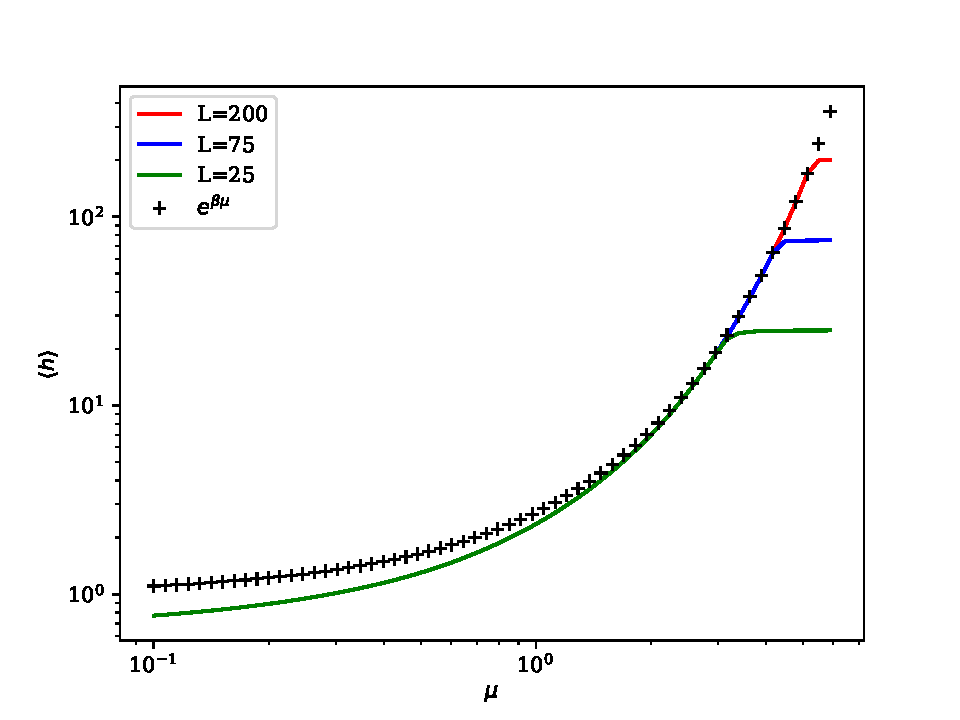
\includegraphics{pop/hauteur-tm-pop.pdf}
\caption{Mean height of the POP model with respect to chemical potential $\mu$ through transfer matrix with different maximal heights in the thermodynamic limit $L'\to \infty$, compared to the Striling's approximation Eq \eqref{stirling-pop},at $\beta=1$. {\color{red} add MC sim}}
\label{haut-tm-pop} 
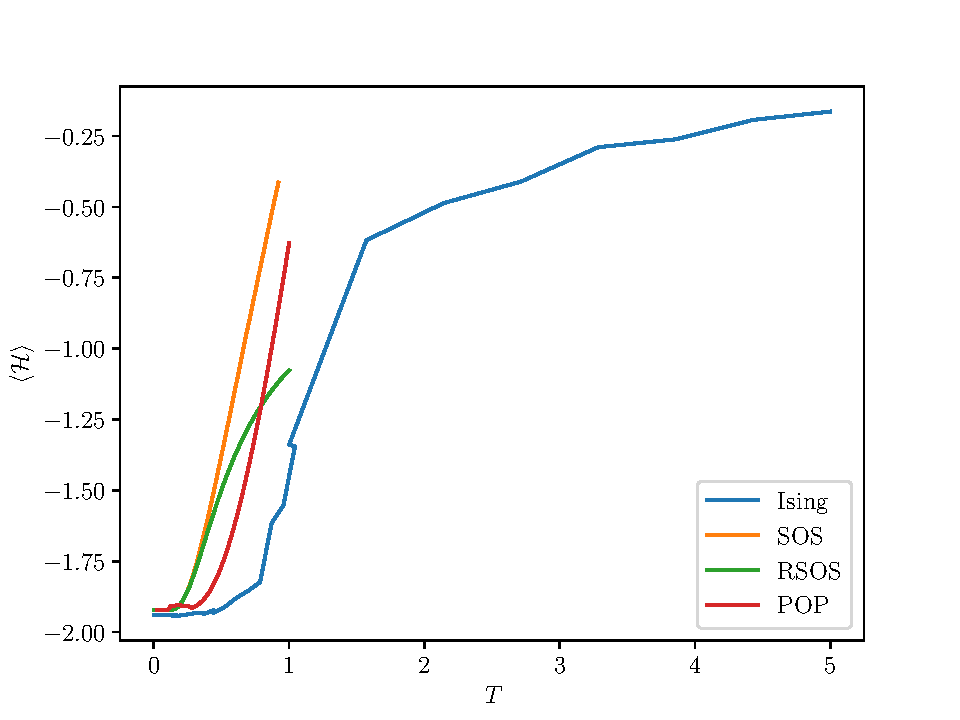
\includegraphics{pop/comparaison-modeles.pdf}
\caption{Comparison of the internal mean total energy of the Ising, SOS, RSOS and POP models with respect to temperature in absence of external field and $\mu=0$, from Monte Carlo simulations at $L'=126$ and $L=30$ with Glauber dynamics. We used Eq \ref{energie-sos-ising} to compare energies between the interface models and the Ising one.
{\color{red} redo sims for Ising, need MCIA, takes too long otherwise}}
\label{comp-models}
\end{figure}

The transfer matrix is
\begin{align}
T_{POP}(h,h') = T_{SOS}(h,h') \exp \left(- \frac{\ln(h)+\ln(h')}{2} \right)
\end{align}

The Monte Carlo implementation is as follows. Each particle is labeled with the site $i$ in which it is, and $h_i$ is the number of particles numbered at that site. 
In the Glauber dynamics, particles can be exchanged with a reservoir. With a probability $1/2$ one attempts to add a particle and with probability $1/2$ one attempts to takeaway a particle. In the first case, a site $i$ is chosen with a uniform distribution, and we attempt to create a new particle labeled at site $i$ with probability $min(1,\exp(-\beta \Delta E))$. In the latter, a particle is selected uniformly between all existing particles, and an attempt to remove it is done
\footnote{In C++, we can use a $std::vector$ in which we add or remove particles. After each success attempt, we rebuild the distribution $std::uniform\_int\_distribution(0,N-1)$, where N is the number of particles. This operation is lightweight and should not cause any slowing down. For the next section's algorithm with multiple particle types, we use $std::discrete\_distribution<>$. }.
Kawasaki dynamics is implemented by randomly choosing a particle $n$ with probability $\frac{1}{N}$ at each Monte Carlo step, then trying to move the particle to the left or right using Metropolis acceptance rate. 

In Fig \ref{comp-models}, we plot the internal energy of the Ising, SOS, RSOS and POP models with respect to temperature in absence of external fields and $\mu=0$ wtih non-conserved dynamics. {\color{red} discuss the graph once plots are better}

Contrary to the SOS model where there needs to be a confining external field in order to localize the interface \cite{burkhardt_localisation-delocalisation_1981,chui_pinning_1981}, the entropic term gives a stable position for the interface. In absence of external field, the effective potential is given by
\begin{align} 
    V_{eff}(h) = - \mu h + \frac{1}{\beta}\ln(h!)
\end{align}
If the chemical potential is large enough, the number of particles $N$ is large enough, so we can use Striling's formula and approximate a continuous derivative with the finite-difference in $h$, so we have
\begin{align} 
    V_{eff}(h)' = - \mu +\frac{1}{\beta} \ln(h)
\end{align}which gives the mean height 
\begin{align} 
    <h> = \exp(\beta \mu) 
\label{stirling-pop}
    \end{align}
    In Fig \ref{haut-tm-pop}, we show the mean height \eqref{stirling-pop} compared to the transfer matrix diagonalisation with different matrix size and the Monte Carlo simulations at$\beta=1$. We see that when $ <h> \gg 1$, the Stirling's formula becomes valid and Eq \eqref{stirling-pop} becomes accurate. Since $<h>$ cannot exceed the maximum size of the system, saturation occurs at large $\mu$. 


%%%%%%%%%%%%%%%%%%%%
    \section{$M$-particles POP system}
%%%%%%%%%%%%%%%%%%%%


\begin{figure}
    \centering
    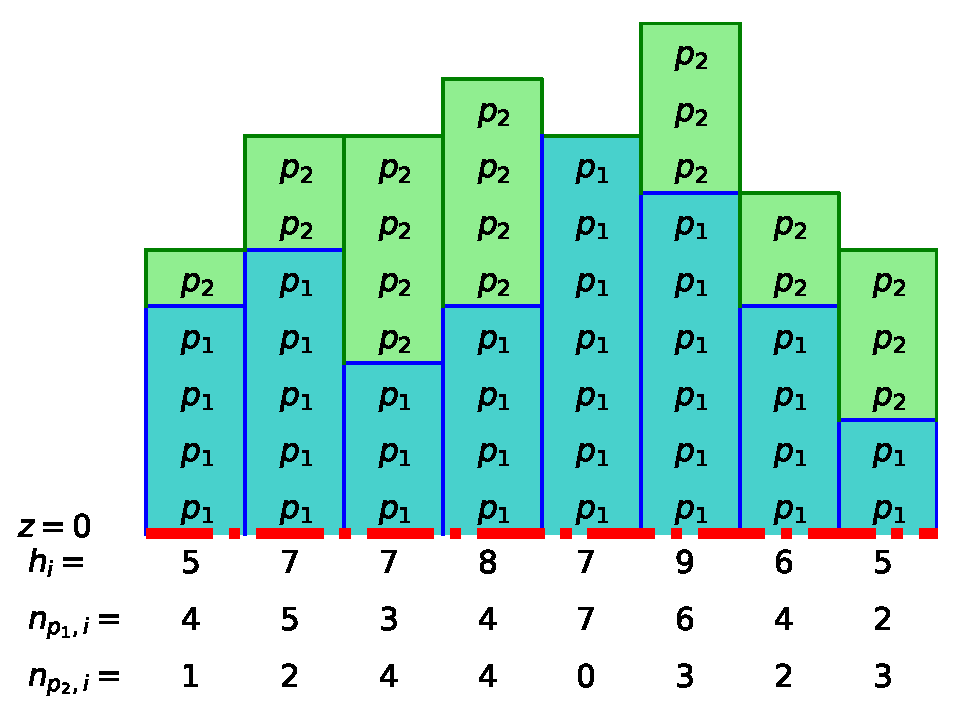
\includegraphics[width=0.7\linewidth]{pop/figure-pop.pdf}
    \caption{Possible POP configuration with two types of particles $p_1$ and $p_2$. The red line shows the origin $z=0$. In the $i$-th column the interface is at height $h_i$, with $n_{1,i}$ particles of type $p_1$ at site $i$, and same for particles $p_2$. Over the interface, there are no particles. }
    \label{fig-pop}
\end{figure}

We consider a model of a surface delimiting a bulk phase of $L'$  sites which contains $M$ different particle types $p_1 ... p_M$, $N_m$ is the total number of particles of type $m$ and $n_{m,i}$ denotes the number of particles of type $m$ at site $i$. The interface height is $h_i = \sum_m n_{m,i}$. Taking into account the entropic contribution, the effective Hamiltonian for the model is
\begin{align}
    H[M] = J \sum_i |h_i-h_{i+1}| + \sum_i V(h_i) - \sum_m \mu_m \sum_i n_{m,i} + \frac{1}{\beta} \sum_m \sum_i \ln(n_{m,i})
    \label{ham-pop-c}
\end{align}
We assume that the particles in each column are demixed, i.e. the permitted particle configurations are taken to be stacked vertically such that the stack of $p_{m+1}$ particles lies on top  of the $p_m$ particles, as seen in Fig \ref{fig-pop} for $M=2$. The first term in the Hamiltonian corresponds to the surface tension with a gas phase above the stacks of particles. As disccused with the SOS model, we can have a restricted or gaussian version of Eq \ref{ham-pop-c}. 

The grand partition function is given by
\begin{align}
    \Xi = \sum_{{\bf n_1...n_M}} \exp(-\beta H[M])
\end{align}

The motivation for a $M$ particle theory is that when one develops a continuous, off latice theory, based on Brownian dynamics, any single particle theory is insensitive to constant driving due to Galilean invariance, the presence of two or more different particle types breaks this invariance and yields non-equilibrum effects.

If $M=2$, the the statics of the above can be reduced to the study of a single particle model by making the change of variable $n_{2,i} = h_i - n_{1,i}$. Using the binomial relation ${(a+b)^{n_1} = \sum_{h'=0}^h \frac{h!}{h'! (h-h')!} a^{h'} b^{h'-h}}$, the sum over the variables $n_{1,i}$ can be trivially carried out and we find
\begin{align}
    \Xi =& \sum_{\bf h} \exp \left( -\beta J \sum_i |h_i-h_{i+1}| - \sum_i \ln(h_i!) + \beta \mu_e \sum_i h_i \right) \nn
    =& \sum_{\bf h} \exp \left( -\beta H_{eff}(h_1,h_2...h_{L'}) \right)
\end{align}
where $\mu_e = \frac{1}{\beta}\ln( \exp(\beta \mu_1) + \exp(\beta \mu_2)$ is the effective chemical potential for the variables $h_i$. If we add a third type of particle, we see clearly see that the same reduction can be carried out. Thus, by recursivity, we can show that for any number of particle type $M$, we have the same effective Hamiltonian as the single particle system \eqref{heff-pop}, with an effective chemical potential
\begin{align}
    \mu_e = \frac{1}{\beta} \ln \left( \sum_m \exp( \beta \mu_m ) \right)
\end{align}
An interesting thing to remark is that even if the chemical potential of a particle type $\mu_m = 0$, its contribution to the effective chemical potential is nonzero. 
This reduced theory can be numerically solved in equilibrium by transfer matrix methods. 

Now let the subset $\bar{M}$ of particle types from the $M$ particle types be in the canonical ensemble, while all the other ones are in the grand-canonical one. {\color{red} which kind of physical systems, put ref from the paper} The total partition function is then
\begin{align}
    \Xi = \sum_h \exp \left( -\beta H_{eff}(h_1,h_2...h_{L'}) \right) \prod_{m \in \bar{M}}  \delta_{\sum_{i=1}^{L'} h_i,N_m}
\end{align}

Mixing Glauber and Kawasaki dynamics for different particle types is implemented using the following algorithm. Each non-conserved particle type posseess a kinetic coefficient $\alpha_m$, while each conserved particle type has a diffusive coefficient $D_m$. We set $p_m = \alpha_m$ is the particle is non-conserved, and $p_m = D_m$ otherwise, and we normalize it in order to have $\sum_m p_m = 1$. At each Monte Carlo step, a particle of type $m$ is chosen with probability $p_m$, and then we proceed with Glauber or Kawasaki dynamics for a single-type particle system, as described in the previous section.
To test the algorithm with a view to studying the driven system, we have implemented it in for two particles types both in the grand-canonical ensemble for the case of no driving and have compared the results with the equilibrium transfer matrix which we carried out numerically. In the case where the dynamics is conserved we compared them to the non-conserved case.

In order to compare the equilibrium calculation to the numerical simulations, we fix the average number of particles $<n_{m,i}>$ at each by
\begin{align}
    < n_m > =& \frac{1}{\beta L'} \frac{\partial}{\partial \mu_m} \ln(\Xi) \nn
    =& \frac{1}{\beta L'} \frac{\partial \mu_e}{\partial \mu_m} \frac{\partial}{\partial \mu_e} \ln(\Xi) \nn
    =& \frac{\exp(\beta \mu_m)}{\sum_m \exp(\beta \mu_m)} <h>
\end{align}
where $<h> = <\sum_m n_m>$. 

%%%%%%%%%%%%%%%%%%%%%%
    \section{Continuum Theory}    
%%%%%%%%%%%%%%%%%%%%%%

In order to understand the statics of the model we write a continuum version of the theory with $M$ field $n_m(x)$  and we take the a Gaussian form for the surface energy
\begin{equation}
H =  \int dx \frac{\sigma}{2} [\frac{d}{dx} (\sum_m n_m)]^2  + V(n_1(x),...,n_M(x))
\end{equation}
where $\sigma$ is the surface tension and 
\begin{equation}
    V(n_1(x),...n_M(x)) = \sum_m -\mu_m n_m(x) + T n_m(x) [ \ln(n_m(x))-1 ]
\end{equation}
We have used Stirlings formula and thus assumed that the typical value of $n_m(x)$ aree large. 
We now expand $V(n_1(x),...n_M(x))$ by writing $n_m(x) = \overline n_m + \phi_m(x)$  where $(\overline n_1,..\overline n_M)$ is the minimum of $V(n_1,..n_M)$. Here we find
\begin{equation}
    \overline n_m = \exp(\beta \mu_m) 
\end{equation}

This gives an effective Hamiltonian for the fluctuations of the fiels  $\phi_m$ 
\begin{equation}
    H_f = \frac{\sigma}{2}\int dx [\frac{d}{dx}(\sum_m \phi_m]^2 + \sum_m r_m \phi_m^2(x) 
\end{equation}
where 
\begin{equation}
    r_m = \frac{T}{\sigma \overline n_m} \
\end{equation}
A straight forward calculation then shows that the Fourier transform of the connected height-height fluctuation correlation function is
\begin{equation}
    \tilde C_{hh}(k) = \frac{T}{\sigma} \frac{1}{k^2 + r_e}
    \label{stat}
\end{equation}
where $r_e = \prod_m r_m/ \sum_m r_m$. We thus find
\begin{equation}
    <h^2>= \frac{T}{2\sigma m_e} = \frac{1}{2}\sqrt{\frac{T\overline h}{\sigma}},
\end{equation}
where $\overline h= \sum_m \overline n_m$.

%%%%%%%%%%%%%%%
    \section{Dynamics of the continuum model for two particles}
%%%%%%%%%%%%%%%

%%%%%%%%%%%%%%%
    \subsection{Conserved diffusive dynamics}
%%%%%%%%%%%%%%%
We now study a system of two particle types $A$ and $B$, where one is a a solvent and the other one a particle in suspension, for example.
Assuming Brownian dynamics for the particles, the stochastic density functional equations for the continuum fields $n_A$ and $n_B$ are
given by
\begin{equation}
\frac{\partial n_A(x)}{\partial t} = \frac{\partial}{\partial x} \beta D_A n_A(x)\frac{\partial}{\partial x} \frac{\delta H}{\delta n_A(x)} + \frac{\partial}{\partial x} \sqrt{2D_A n_A(x)} \eta_A(x,t)
\end{equation}
and 
\begin{equation}
\frac{\partial n_B(x)}{\partial t} = \frac{\partial}{\partial x} \beta D_B n_B(x)\frac{\partial}{\partial x} \frac{\delta H}{\delta n_B(x)} + \frac{\partial}{\partial x} \sqrt{2D_Bn_B(x)} \eta_B(x,t)
\end{equation}
where $D_A$ and $D_B$ are the diffusion constants of the particles. The noise terms are independent , zero mean, spatiotemporal Gaussian white noise with
\begin{eqnarray}
\langle \eta_A(x,t) \eta_A(x',t')\rangle = \langle \eta_B(x,t) \eta_B(x',t')\rangle =\delta(x-x')\delta(t-t').
\end{eqnarray}
As we are interested in what happens when one of the species is driven, we add a term
\begin{equation}
H_D = -\int dx xf n_A(x)
\end{equation}
to the Hamiltonian, this corresponds to a force which pushes the particles of type $A$ to the right. We also assume periodic boundary conditions, and thus a current will exist in the resulting steady state.
This introduces term in the equation for $n_A(x)$ which becomes
\begin{equation}
\frac{\partial n_A(x)}{\partial t}+ \frac{\partial}{\partial x}D_A\beta f n_A(x) = \frac{\partial}{\partial x} \beta D_A n_A(x)\frac{\partial}{\partial x} \frac{\delta H}{\delta n_A(x)} + \frac{\partial}{\partial x} \sqrt{2D_A n_A(x)} \eta_A(x,t).
\end{equation}
It is important to note that in the absence of the particles of type $B$, the resulting equation for the field $n_A(x,t)$ can be rendered independent of
the force $f$ via the Galilean transformation
\begin{equation}
n(x,t) = n(x-vt,t)
\end{equation}
where $v= D_A\beta f$ is the induced drift on the particles of type $A$.
Note that the Galilean invariance can also be broken if the force $f$ acts on both particle types but the diffusion coefficients $D_A$ and $D_B$ are different.

We now expand the deterministic part of the two equations to first order in the density fluctuations about its mean value and the noise terms to zeroth order. This approximation respects detailed balance for the effective quadratic Hamiltonian and has been used with accuracy in a wide variety of contexts. The resulting dynamics of of a model B and Fourier transforming in space gives
\begin{equation}
\frac{\partial \tilde{\boldmath \Phi}(k,t)}{\partial t}= -\beta \tilde A(k){\boldmath \Phi}(k,t) + {\boldmath \tilde\eta}(k,t),
\end{equation}
where
\begin{equation}
{\boldmath \Phi}(k,t) =\begin{pmatrix} &\tilde \phi_A(k,t) \\ &\tilde \phi_B(k,t)\end{pmatrix}
\end{equation}
The noise correlation function is given by
\begin{equation}
\langle {\tilde\boldmath\eta}^{T}(k,t) {\tilde\boldmath{\eta}}(k',t')\rangle = 4\pi\tilde R(k) \delta(t-t')\delta(k+k')
\end{equation}
where 
\begin{equation}\tilde R(k)= 2\begin{pmatrix} & D_A\overline n_A k^2 & 0\\
& 0 & D_B\overline n_B k^2\end{pmatrix},
\end{equation}
and 
\begin{equation}
\tilde A(k) =\sigma\begin{pmatrix}& D_A\overline n_A k^2(k^2 + m_A^2) -i\frac{D_A k f}{\sigma} & 
D_A\overline n_A k^4 \\ & D_B\overline n_B k^4 & D_B \overline n_B k^2(k^2 + m_B^2).\end{pmatrix}
\end{equation}
The Fourier transform steady state correlation function matrix defined by
\begin{equation}
\langle {\boldmath\tilde\Phi}^T(k){\boldmath\tilde\Phi}(k')\rangle =
2\pi \delta(k+k') \tilde C(k)
\end{equation}
is then given by the solution to the Lyapounov equation
\begin{equation}
\tilde A(k)\tilde C(k) + \tilde C(k)\tilde A^T(-k) = 2T \tilde R(k).
\end{equation}
Solving this we find that
\begin{equation}
\tilde C_{hh}(k)= \frac{T}{\sigma}\frac{k^2(m_A^2+m_B^2)(D_A\overline n_A[k^2+m_A^2] +D_B\overline n_B[k^2+m_B^2] )^2 +\frac{f^2 }{\sigma^2}D_A^2(2k^2+m_A^2 + m_B^2)}{k^2(D_A\overline n_A[k^2+m_A^2] +D_B\overline n_B[k^2+m_B^2] )^2(m_A^2 m_B^2 + k^2(m_A^2 +m_B^2))
+\frac{f^2 }{\sigma^2}D_A^2(k^2+m_A^2)(k^2+m_B^2)}.
\end{equation}
In the equilibrium or non-driven system where $f=0$ the above formula
yields the static result Eq. (\ref{stat}). Of particular interest is the strong driving limit where we find that as $f\to\infty$ the result
\begin{equation}
\tilde C_{hh}(k)=\frac{T}{\sigma}\left[\frac{1}{k^2+m_A^2}
+\frac{1}{k^2+m_B^2}\right]
\end{equation}
The effect of strong  driving is to decouple the fluctuations of $n_A$ and $n_B$ and we see that the total height fluctuation is that of the sum two independent interfaces. The height variance is then given by
\begin{equation}
\langle h^2\rangle_s = \frac{T}{2\sigma m_d}
\end{equation}
where 
\begin{equation}
m_d = \frac{m_A m_B}{m_A+m_B}
\end{equation}
From this we find that
\begin{equation}
\frac{\langle h^2\rangle_s }{\langle h^2\rangle_{eq}}=\frac{m_A+m_B}{\sqrt{m_A^2 + m_B^2}}.
\end{equation}
We also see that, as $m_A$ and $m_B$ are positive, the fluctuations in limit of infinite driving are always larger than in the equilibrium state. 


Imagine now that the $B$ particles constitute the bottom layer and that $D_B\ll D_A$ this mimics the solid on solid dynamics where only the top layer of the particles participate in the dynamics. This gives
\begin{equation}
\tilde C_{hh}(k)= \frac{T}{\sigma}\frac{k^2(m_A^2+m_B^2)(\overline n_A[k^2+m_A^2] )^2 +\frac{f^2 }{\sigma^2}(2k^2+m_A^2 + m_B^2)}{k^2(\overline n_A[k^2+m_A^2]  )^2(m_A^2 m_B^2 + k^2(m_A^2 +m_B^2))
+\frac{f^2 }{\sigma^2}(k^2+m_A^2)(k^2+m_B^2)}.
\end{equation}
Assuming the $A$ layer is thinner that the $B$ layer so $m_B\ll m_A$ gives
\begin{equation}
\tilde C_{hh}(k)= \frac{T}{\sigma}\frac{k^2 m_A^2(\overline n_A[k^2+m_A^2] )^2 +\frac{f^2 }{\sigma^2}(2k^2+m_A^2 )}{k^2(\overline n_A[k^2+m_A^2]  )^2(m_A^2 m_B^2 + k^2 m_A^2)
+\frac{f^2 }{\sigma^2}(k^2+m_A^2)(k^2+m_B^2)}.
\end{equation}
which simplifies to give
\begin{eqnarray}
\tilde C_{hh}(k)&=& \frac{T}{\sigma}\frac{k^2 m_A^2(\overline n_A[k^2+m_A^2] )^2 +\frac{f^2 }{\sigma^2}(2k^2+m_A^2 )}{(k^2+m_A^2)(k^2 + m_B^2)[(n_A^2m_A^2 k^2(k^2+m_A^2)
+\frac{f^2 }{\sigma^2}]} \\
\tilde C_{hh}(k)&=& \frac{T}{\sigma}\frac{1}{k^2 + m_B^2}
+\frac{T}{\sigma}\frac{\frac{f^2 }{\sigma^2}k^2}{(k^2+m_A^2)(k^2 + m_B^2)[(n_A^2m_A^2 k^2(k^2+m_A^2)
+\frac{f^2 }{\sigma^2}]} 
\\
&=&\frac{T}{\sigma}\left[\frac{1}{(k^2 + m_B^2)}
+\frac{ f^2 }{\sigma^2\overline n_A^2 m_A^2}\frac{k^2}{(k^2+m_A^2)(k^2 + m_B^2)(k^4+m_A^2 k^2 +\frac{f^2 }{\sigma^2n_A^2 m_A^2})}\right]
\end{eqnarray}
The height fluctuations are then given by
\begin{equation}
\langle h^2\rangle = \frac{T}{2\sigma m_B} +  \frac{T}{2\sigma}\frac{ f^2 }{\sigma^2\overline n_A^2 m_A^2}\frac{m_A + m_B+ m_++ m_-}{(m_A+m_B) (m_++m_B)(m_-+m_B)(m_A+m_+)(m_A+m_+)(m_++m_-)},
\end{equation}
where 
\begin{equation}
m_\pm = \sqrt{\frac{m_A^2\pm\sqrt{m_A^4 -\frac{4f^2 }{\sigma^2n_A^2 m_A^2}}}{2}}
\end{equation}

%%%%%%%%%%%%%%%
    \subsection{Non conserved dynamics}
%%%%%%%%%%%%%%%
We now consider the case where the particles of type $B$ are in contact with 
a reservoir of the same particles in a vapour phase. To model this we modify the dynamics of the B phase by introducing a component of non-conserved dynamics for these particles
\begin{equation}
\frac{\partial n_B(x)}{\partial t} = \frac{\partial}{\partial x} \beta D_B n_B(x)\frac{\partial}{\partial x} \frac{\delta H}{\delta n_B(x)} + \frac{\partial}{\partial x} \sqrt{2D_Bn_B(x)} \eta_B(x,t)
-K_B\beta \frac{\delta H}{\delta n_B(x)} + \sqrt{2K_B}\eta'_B(x,t),
\end{equation}
here if $\eta'_B(x,t)$ is a new spatio-temporal white noise independent of the 
others, the undriven system obeys detailed balance.  Now the average value of the $n_B$ is determined by taking the average in the steady state. As the system is invariant under translation, the average of the first diffusive term on the right-hand-side is zero and so we find
\begin{equation}
\langle \frac{\delta H}{\delta n_B(x)}\rangle=0,
\end{equation}
where the averaging is over the system in the steady state. Again invariance by translation in space can be applied to write
\begin{equation}
\langle \frac{\partial V(n_A,n_B)}{\partial n_A}\rangle  =0
\end{equation}
Here we have $V(n_A,n_B)= U(n_A) + U(n_B)$ where $U(x) = Tx(\ln(x)-1)-\mu x$ and so expanding about $\overline n_A$ we find to second order that 
\begin{equation}
\langle U'(\overline n_A) + U''(\overline n_A)\phi_A +\frac{1}{2}U'''(\overline n_A)\phi_A ^2 \rangle =0,
\end{equation}
the equation to first order gives 
\begin{equation}
U'(\overline n_A)=0
\end{equation}
which gives $\overline n_A= n_m$ where $n_m$ is the value for which $U$ attains its minimum. However if we keep the next order term we find 
\begin{equation}
U'(\overline n_A)+\frac{1}{2} U'''(\overline n_A)\langle\phi_A ^2 \rangle=0.
\end{equation}
If the renormalization of the average value of $\overline n_A$ is assumed to be small we can write
\begin{equation}
\overline n_A= n_m +\delta,
\end{equation}
which gives
\begin{equation}
\delta = -\frac{1}{2} \frac{U'''(n_m)}{U''(n_m)}\langle\phi_A ^2 \rangle.
\end{equation}
For the (entropic) potential in question here we have
\begin{equation}
\delta = \frac{1}{2n_m} \langle\phi_A ^2 \rangle,
\end{equation}
we thus see that the average height of the interface is increased due to fluctuations. The non-equilibrium fluctuations are stronger an thus the height increases under driving. 

              
              
              

